\chapter{Reproducibility}
\label{app:repro}

\begin{sloppypar}

This appendix lists what is in the code folder, the order in which the scripts run, and the environment they ran in. Everything the dissertation quotes is produced by one of these scripts and written to a JSON file; the numbers and tables in the text are generated from those files by \texttt{export\_tex.py}.

\section{Repository layout}
\begin{itemize}\setlength{\itemsep}{1pt}
\item \texttt{emoviz/emoviz/metrics.py}: the only definition of every measure, split rule, centroid and the random-pairing null. Every other script imports it.
\item \texttt{emoviz/emoviz/data.py}: the loader. It resolves the three filename schemes, reads the signing timestamps, computes prompt groups and applies name redaction at load time.
\item \texttt{emoviz/preprocess\_names.py}: the three-stage redaction procedure (detect, review, apply). The reviewed decision table is kept with the dataset, not with the code.
\item \texttt{emoviz/describe\_extract.py}: the pipeline (BLIP-VQA, the template, BART-MNLI). It checkpoints to a JSONL file after every record and resumes from it.
\item \texttt{emoviz/analysis\_final.py}: the splits, the four measures, the nulls and the distinct-prompt re-run. Writes \texttt{outputs/analysis\_final.json}.
\item \texttt{emoviz/significance.py}: the clustered bootstrap and the clustered permutation test of the face/scene difference.
\item \texttt{emoviz/inference.py}: clustered intervals for every subset, Cohen's $\kappa$, the Holm procedure, and the seed check on $z$.
\item \texttt{emoviz/method\_comparison.py}: the like-for-like comparison of the two image readers with the paired tests.
\item \texttt{emoviz/data\_audit\_consistency.py}: the record accounting and the repeated-prompt consistency with its permutation null.
\item \texttt{emoviz/audits.py}: the control audit, the describer audit and copy rate, and per-family recall.
\item \texttt{emoviz/error\_taxonomy.py}: the census of high-confidence disagreements and their failure modes.
\item \texttt{emoviz/ablate\_nli.py}: the description-template ablation (only the entailment stage re-runs).
\item \texttt{emoviz/human\_check.py}: draws the single-coder sample, lays out the contact sheets, and scores the coded file.
\item \texttt{emoviz/make\_figures.py} and \texttt{emoviz/export\_tex.py}: every figure, and every number and table in this document, from the JSON files. The four extra figures in this document are made by \texttt{dissertation/build\_notes/make\_extra\_figures.py}.
\item \texttt{emoviz/app.py} and \texttt{emoviz/web/}: the demonstrator.
\item \texttt{emoviz/test.sh} and \texttt{emoviz/test\_numeric.py}: the smoke suite and the pinned numeric checks.
\item \texttt{emoviz/outputs/}: cached model outputs, the result JSON files, the figures, and the frozen direct-CLIP file.
\end{itemize}

\section{Run order}
\begin{enumerate}\setlength{\itemsep}{1pt}
\item \texttt{bash emoviz/setup.sh} creates the environment from the pinned \texttt{requirements.txt}.
\item \texttt{describe\_extract.py} runs the pipeline over all images. Its output is cached, so this step is only repeated to regenerate from scratch.
\item \texttt{analysis\_final.py} runs the main analysis from the cached outputs in a few seconds.
\item \texttt{significance.py}, \texttt{inference.py} and \texttt{method\_comparison.py}.
\item \texttt{data\_audit\_consistency.py}, \texttt{audits.py}, \texttt{error\_taxonomy.py} and \texttt{ablate\_nli.py} (the ablation takes about half an hour because it re-runs the entailment model).
\item \texttt{human\_check.py sample}, then code \texttt{outputs/human\_check/labels.csv} from the sheets, then \texttt{human\_check.py score}.
\item \texttt{make\_figures.py} and \texttt{export\_tex.py}, then build this document with \texttt{pdflatex}, \texttt{bibtex}, and \texttt{pdflatex} twice more.
\item \texttt{bash emoviz/test.sh} runs everything above that is fast, plus \texttt{test\_numeric.py}.
\end{enumerate}
All scripts are run with \texttt{emoviz/.venv/bin/python} from the \texttt{emoviz/} directory. The dataset folder sits next to \texttt{emoviz/} and is never copied or uploaded.

\section{Environment}
Python 3.12 with PyTorch 2.13 and Transformers 5.14, on an Apple-silicon laptop with 16~GB of memory; the models run on the Metal backend in half precision. The models are \texttt{SamLowe/roberta-base-go\_emotions} (about 125 million parameters), \texttt{Salesforce/blip-vqa-base} (about 385 million), \texttt{facebook/bart-large-mnli} (about 407 million) and OpenCLIP ViT-B/32 with LAION-2B weights for the comparison reader. The first run downloads about 3.5~GB of weights. The pipeline processed all \nTotal\ images without an unhandled error, which is a statement about robustness and not about correctness; the per-record time was between about one and twelve seconds, slowing when memory was short. Every random process is seeded (the analysis seed is \nullSeed).

\begin{figure}[htbp]
\centering
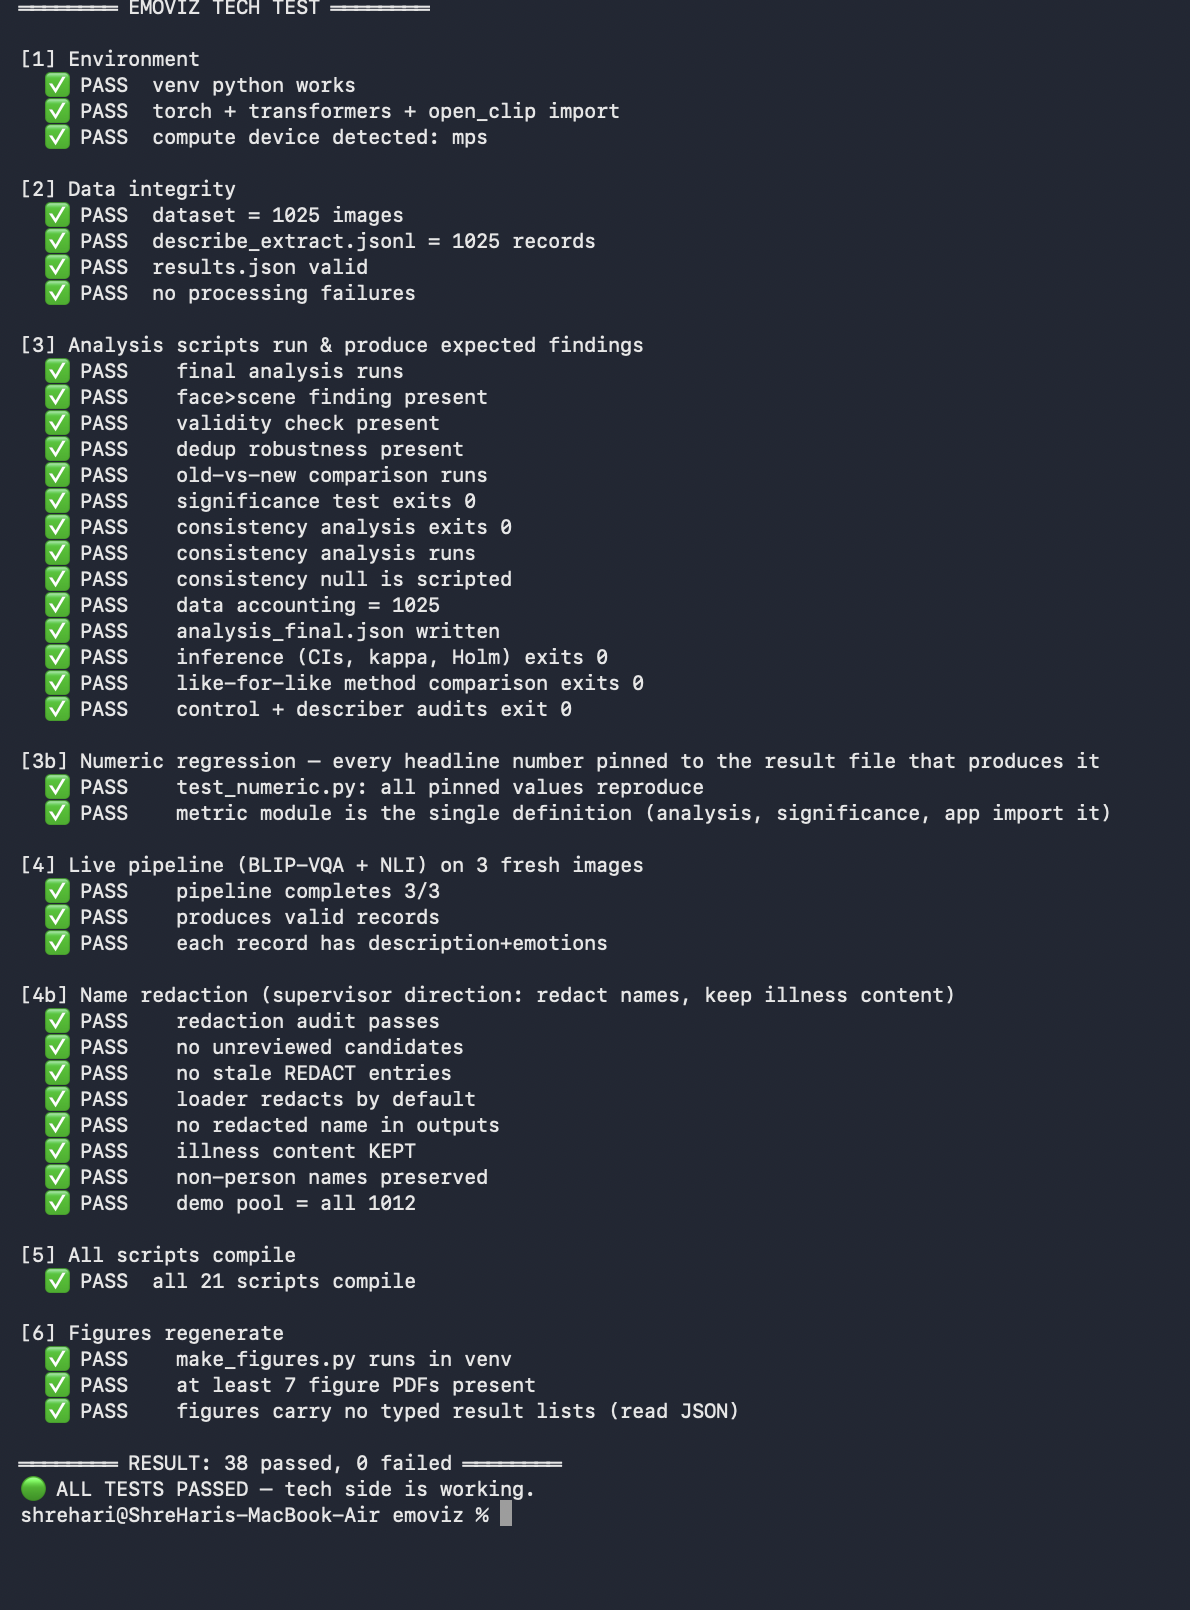
\includegraphics[width=0.82\textwidth]{test_suite}
\caption{The automated self-test after a full run (\texttt{bash emoviz/test.sh}): the environment and data checks, every analysis script run to a clean exit, the pinned numeric regression, the live pipeline over three fresh images, the redaction audit, and the figures rebuilt from the result files.}
\label{fig:testsuite}
\end{figure}

\end{sloppypar}
